\chapter{Implementation - Sprint 1}
\section{Usability Test}
We have taken an Usability Test using a group of 5 users. The Usability Test is divided into two sections included (SPSS for Student and SPSS for SPSO). For each section, we want to have feedbacks of participants for the UI of the system and research their experience by using multiple choice questions. We use figma prototype as an object to experience. The link of figma prototype has been provided above.
\subsection{SPSS for Student}
\begin{enumerate}
    \item \textbf{LOGIN PAGE} \\
    In this question, we research the behavior of participants in using LOGIN PAGE.
\begin{figure}[!h]
    \centering
    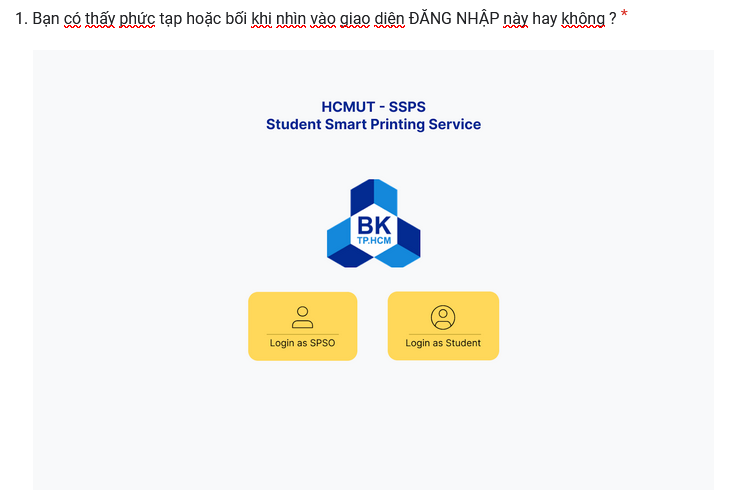
\includegraphics[width=0.8\linewidth]{images/image_uasbility/Q1_Stu.png}
    \caption{LOGIN PAGE}
    \label{fig:LOGIN PAGE}
\end{figure}
\newpage
According to the survey, there are 40\% of participants find it a little curious to understand this task.
\begin{figure}[!h]
    \centering
    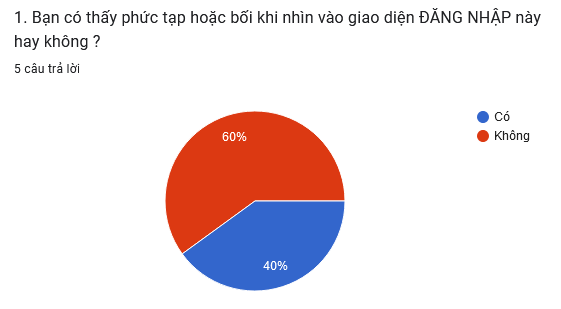
\includegraphics[width=0.8\linewidth]{images/image_uasbility/A1_Stu.png}
    \caption{Char illustrates the result of Question 1}
    \label{fig:Chat illustrates the results of Question 1}
\end{figure}

    \item \textbf{DASHBOARD PAGE} \\
    In this Question, we research the behavior of participants in using DASHBOARD PAGE.
\begin{figure}[!h]
    \centering
    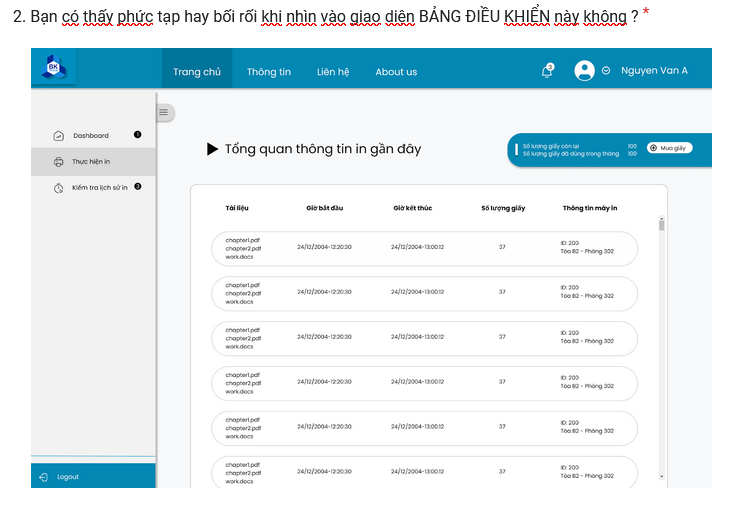
\includegraphics[width=0.8\linewidth]{images/image_uasbility/Q2_Stu.png}
    \caption{DASHBOARD PAGE}
    \label{fig:DASHBOARD}
\end{figure}
\newpage
According to the survey, there are 40\% of participants find it a little curious to understand this task.
\begin{figure}[!h]
    \centering
    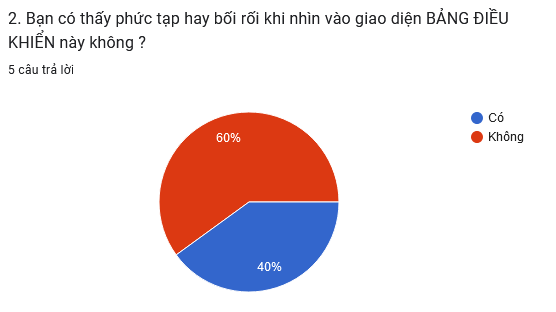
\includegraphics[width=0.8\linewidth]{images/image_uasbility/A2_Stu.png}
    \caption{Chart illustrates the result of Question 2}
    \label{fig:Chart illustrates the result of Question 2}
\end{figure}

    \item \textbf{PRINTING PAGE} \\
    In this Question, we research the behavior of participants in using PRINTING PAGE.
\begin{figure}[!h]
    \centering
    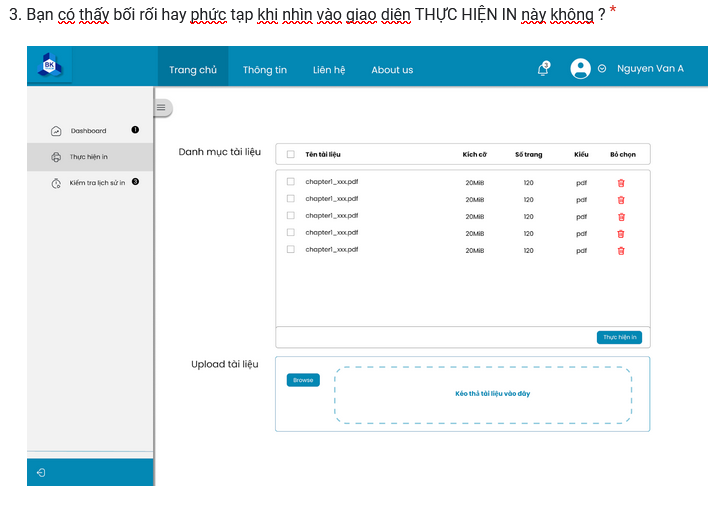
\includegraphics[width=0.8\linewidth]{images/image_uasbility/Q3_Stu.png}
    \caption{PRINTING PAGE}
    \label{fig:PRINTING PAGE}
\end{figure}
\newpage
According the survey, there are 40\% of participants find it a little curious to understand this task.
\begin{figure}[!h]
    \centering
    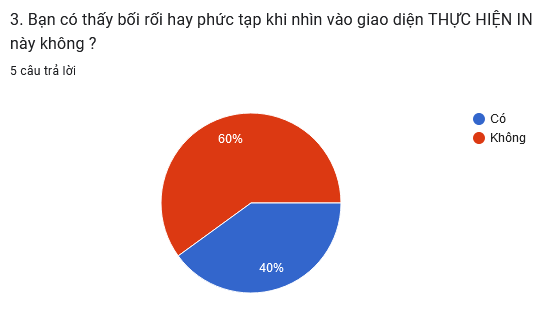
\includegraphics[width=0.8\linewidth]{images/image_uasbility/A3_Stu.png}
    \caption{Chart illustrates the result of Question 3}
    \label{fig:Chart illustrates the result of Question 3}
\end{figure}

    \item \textbf{PRINTING CONFIGURATION PAGE} \\
    In this Question, we research the behavior of participants in using PRINTING CONFIGURATION PAGE.
\begin{figure}[!h]
    \centering
    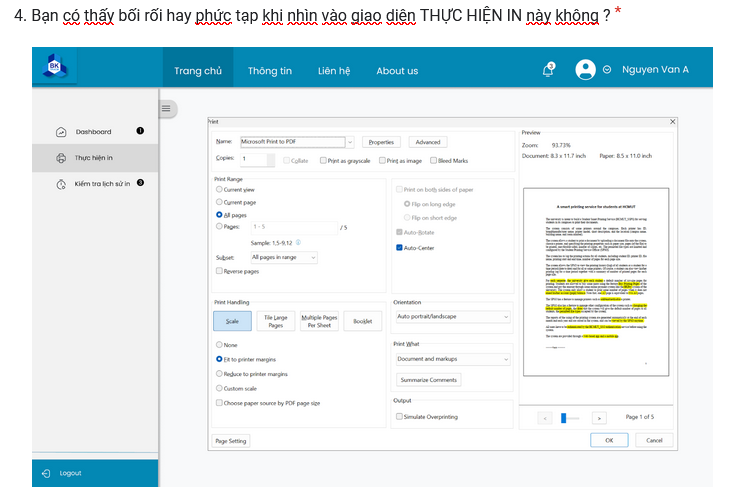
\includegraphics[width=0.8\linewidth]{images/image_uasbility/Q4_Stu.png}
    \caption{PRINTING CONFIGURATION PAGE}
    \label{fig:PRINTING CONFIGURATION PAGE}
\end{figure}
\newpage
According the survey, there are 40\% of participants find it a little curious to understand this task.
\begin{figure}[!h]
    \centering
    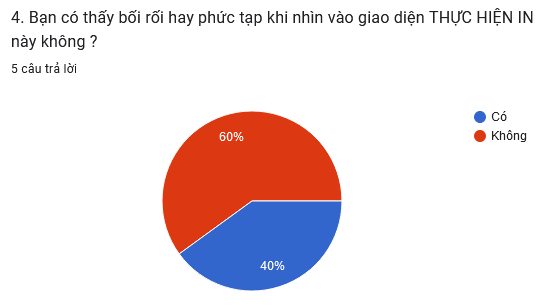
\includegraphics[width=0.8\linewidth]{images/image_uasbility/A4_Stu.png}
    \caption{Chart illustrates the result of Question 4}
    \label{fig:Chart illustrates the result of Question 4}
\end{figure}

    \item \textbf{HISTORY LOG PAGE} \\
    In this Question, we research the behavior of participants in using HISTORY LOG PAGE.
\begin{figure}[!h]
    \centering
    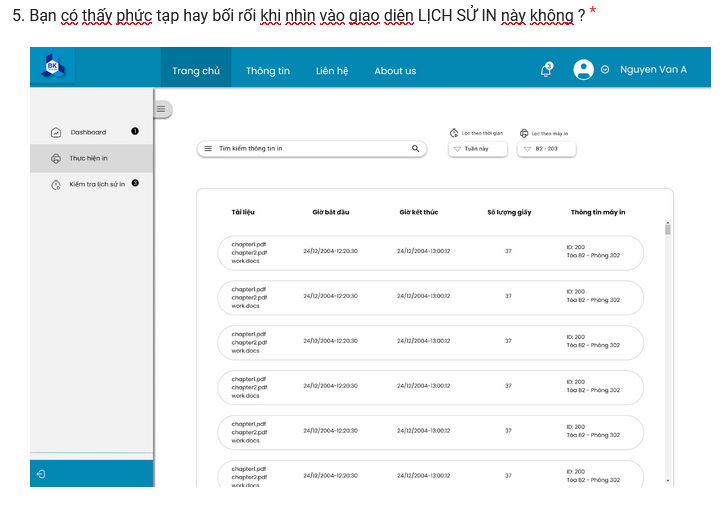
\includegraphics[width=0.8\linewidth]{images/image_uasbility/Q5_Stu.png}
    \caption{HISTORY LOG PAGE}
    \label{fig:HISTORY LOG PAGE}
\end{figure}
\newpage
According the survey, there are 40\% of participants find it a little curious to understand this task.
\begin{figure}[!h]
    \centering
    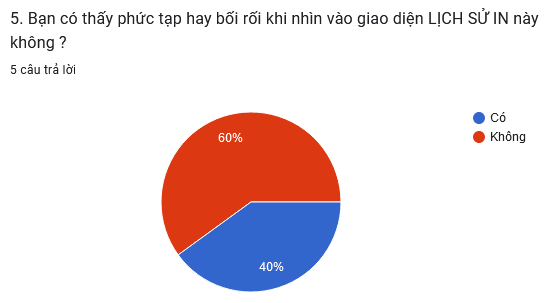
\includegraphics[width=0.8\linewidth]{images/image_uasbility/A5_Stu.png}
    \caption{Chart illustrates the result of Question 5}
    \label{fig:Chart illustrates the result of Question 5}
\end{figure}
\end{enumerate}

\subsection{SPSS for SPSO}
\begin{enumerate}
    \item \textbf{LOGIN PAGE} \\
    In this question, we research the behavior of participants in using LOGIN PAGE.
\begin{figure}[!h]
    \centering
    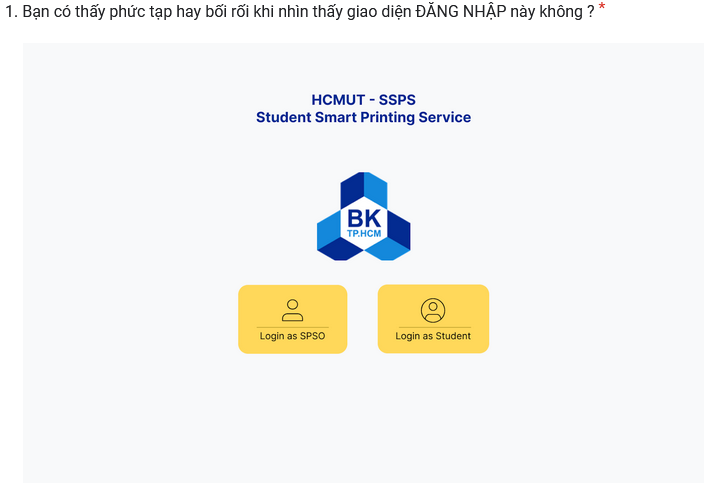
\includegraphics[width=0.8\linewidth]{images/image_uasbility/Q1_SPSO.png}
    \caption{LOGIN PAGE}
    \label{fig:LOGIN PAGE}
\end{figure}
\newpage
According to the survey, there are 60\% of participants find it a little curious to understand this task.
\begin{figure}[!h]
    \centering
    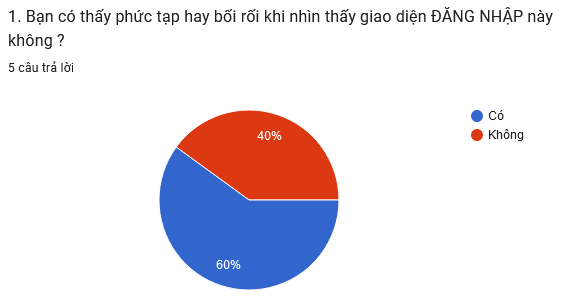
\includegraphics[width=0.8\linewidth]{images/image_uasbility/A1_SPSO.png}
    \caption{Char illustrates the result of Question 1}
    \label{fig:Chat illustrates the results of Question 1}
\end{figure}


    \item \textbf{DASHBOARD PAGE} \\
    In this Question, we research the behavior of participants in using DASHBOARD PAGE.
\begin{figure}[!h]
    \centering
    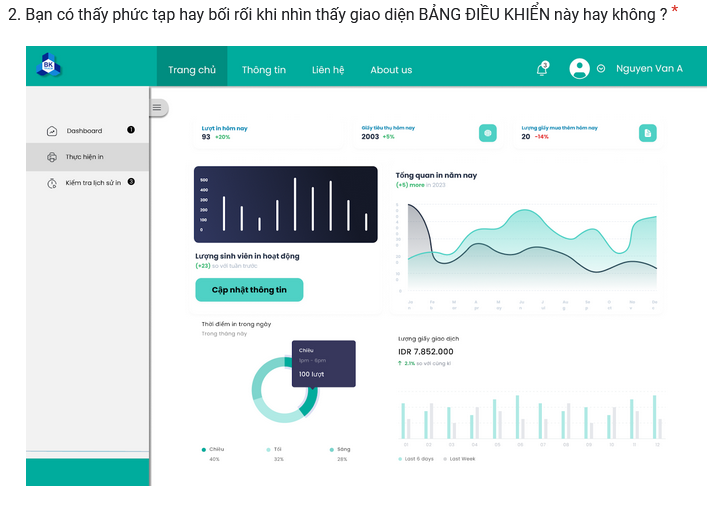
\includegraphics[width=0.8\linewidth]{images/image_uasbility/Q2_SPSO.png}
    \caption{DASHBOARD PAGE}
    \label{fig:DASHBOARD}
\end{figure}
\newpage
According to the survey, there are 60\% of participants find it a little curious to understand this task.
\begin{figure}[!h]
    \centering
    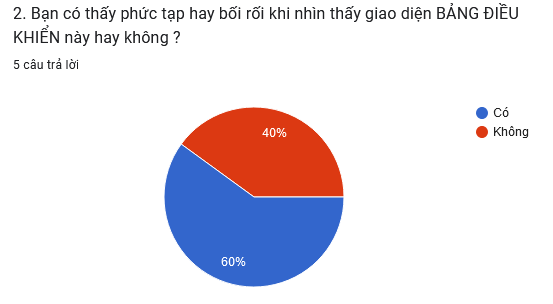
\includegraphics[width=0.8\linewidth]{images/image_uasbility/A2_SPSO.png}
    \caption{Chart illustrates the result of Question 2}
    \label{fig:Chart illustrates the result of Question 2}
\end{figure}


    \item \textbf{PRINTING CONFIGURATION PAGE} \\
    In this Question, we research the behavior of participants in using PRINTING CONFIGURATION PAGE.
\begin{figure}[!h]
    \centering
    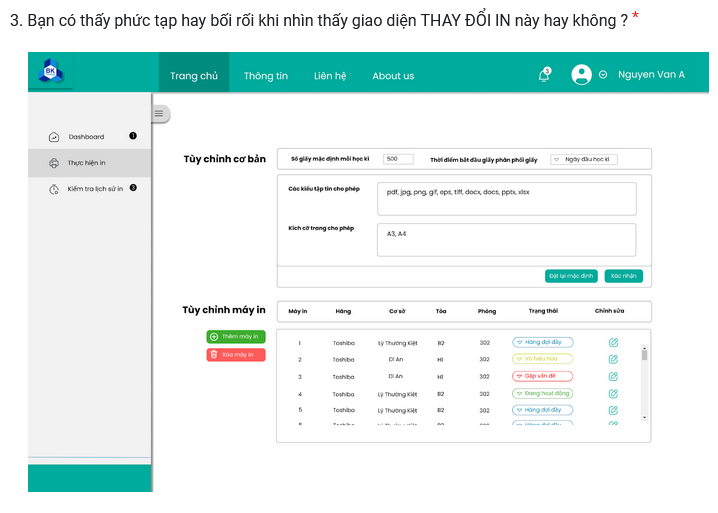
\includegraphics[width=0.8\linewidth]{images/image_uasbility/Q3_SPSO.png}
    \caption{PRINTING CONFIGURATION PAGE}
    \label{fig:PRINTING CONFIGURATION}
\end{figure}
\newpage
According the survey, there are 60\% of participants find it a little curious to understand this task.
\begin{figure}[!h]
    \centering
    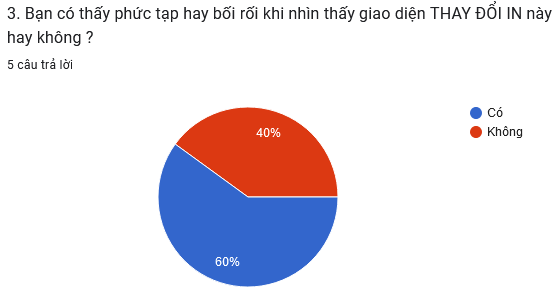
\includegraphics[width=0.8\linewidth]{images/image_uasbility/A3_SPSO.png}
    \caption{Chart illustrates the result of Question 3}
    \label{fig:Chart illustrates the result of Question 3}
\end{figure}


    \item \textbf{HISTORY LOG PAGE} \\
    In this Question, we research the behavior of participants in using HISTORY LOG PAGE.
\begin{figure}[!h]
    \centering
    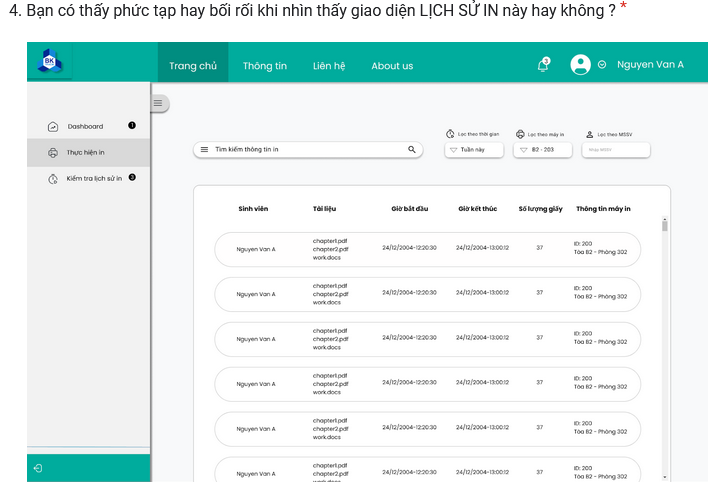
\includegraphics[width=0.8\linewidth]{images/image_uasbility/Q4_SPSO.png}
    \caption{HISTORY LOG PAGE}
    \label{fig:HISTORY LOG PAGE}
\end{figure}
\newpage
According the survey, there are 20\% of participants find it a little curious to understand this task.
\begin{figure}[!h]
    \centering
    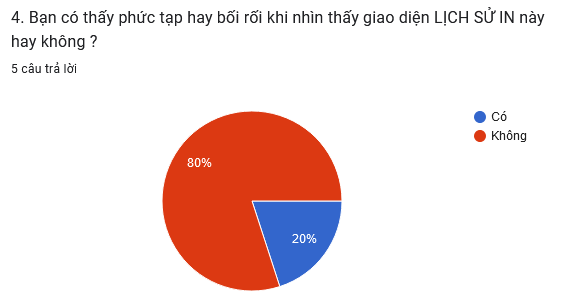
\includegraphics[width=0.8\linewidth]{images/image_uasbility/A4_SPSO.png}
    \caption{Chart illustrates the result of Question 4}
    \label{fig:Chart illustrates the result of Question 4}
\end{figure}
\end{enumerate}

\newpage
